\documentclass[border=10pt]{standalone}
\usepackage{pgfplots}
\pgfplotsset{compat=1.18}
\begin{document}
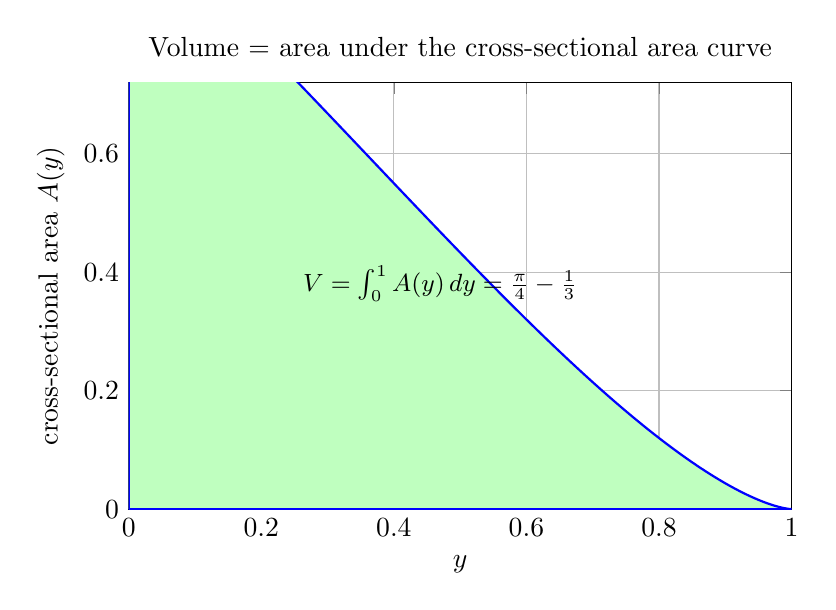
\begin{tikzpicture}
\begin{axis}[
    width=10cm, height=7cm,
    xmin=0, xmax=1, ymin=0, ymax=0.72,
    xlabel={$y$}, ylabel={cross-sectional area $A(y)$},
    title={Volume = area under the cross-sectional area curve},
    domain=0:1, samples=200,
    grid=both,
]
\addplot[fill=green!25, draw=blue, thick] {(1-x)*sqrt(1-x^2)} \closedcycle;
\node[font=\small] at (axis cs:0.47,0.38) {$V=\int_0^1 A(y)\,dy=\frac{\pi}{4}-\frac{1}{3}$};
\end{axis}
\end{tikzpicture}
\end{document}